\documentclass{beamer}
\special{landscape}


\usepackage{ulem}
%\usetheme{Berlin}
%\usetheme{Warsaw}
\usetheme{Boadilla}

%\usecolortheme{seahorse}
%\usefonttheme[onlysmall]{structurebold}

\setbeamertemplate{headline}[split]
\setbeamertemplate{footline}[default]
\setbeamertemplate{footline}[miniframes theme]
%\logo{\includegraphics[scale=0.25]{lifia_logo.png}}

\mode<presentation>
\usepackage[spanish]{babel}
\usepackage{beamerthemesplit}
\usepackage[utf8]{inputenc}
\usepackage{color}      % use if color is used in text


% Comandos en modo Verbatim
%\usepackage{fancyvrb}


\title{Practica 2 - PIO}


\AtBeginSection[]

\begin{document}

\begin{frame}
%\frametitle{Presentación}
\titlepage
\end{frame}

\section{PIO}
\subsection{Introducción}
\begin{frame}
\frametitle{PIO}
%\begin{block}{Slot Accounting System}
\begin{itemize}
 \item Significa Entrada / Salida Programable
 \item VonSim posee 2 puertos de entrada/salida de proposito general:
 \begin{itemize}
   \item Cada puerto es independiente y los llamamos puerto A y B
   \item Cada puerto es de 8 bits 
   \item Cada bit de cada puerto se puede configurar individualmente:
   \begin{itemize}
     \item para entrada: ejemplo, la impresora nos marca que no hay papel
     \item para salida: ejemplo, queremos encender un led
   \end{itemize}
 \end{itemize}
\end{itemize}
\begin{block}{}
Notar que la noción de entrada y salida es relativa a la CPU
\end{block}
\end{frame}

\subsection{Direccionamiento}
\begin{frame}
\frametitle{Direccionamiento}
%\begin{block}{Slot Accounting System}
\begin{itemize}
 \item La dirección base del PIO es 30h
 \item Posee 4 registros de 8 bits
 \begin{itemize}
   \item \emph{PA} (30h): Puerto de Datos A
   \item \emph{PB} (31h): Puerto de Datos B
   \item \emph{CA} (32h): Puerto de Control Puerto A
   \item \emph{CB} (33h): Puerto de Control Puerto B
 \end{itemize}
 \end{itemize}
\begin{center}
 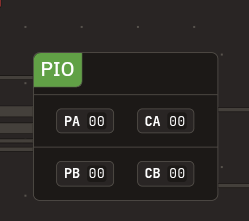
\includegraphics[scale=0.50]{pio_vonsim.png}
\end{center}
%\end{block}
\end{frame}

\subsection{Puertos de Control}
\begin{frame}
\frametitle{Puertos de Control}
%\begin{block}{Slot Accounting System}
\begin{itemize}
 \item Los puertos de control nos permiten configurar como vamos a usar el puerto de datos
 \item Cada bit del puerto de control configura el mismo bit del puerto de datos
 \begin{itemize}
   \item Si ese bit está en 0: el bit del puerto de datos será utilizado para salida
   \item Si ese bit está en 1: el bit del puerto de datos será utilizado para entrada
 \end{itemize}
\end{itemize}

%\end{block}
\end{frame}

\subsection{Conexión en el simulador}
\begin{frame}
\frametitle{Conexión en el simulador}
\begin{itemize}
  \item El simulador permite conectar el PIO de dos maneras diferentes:
  \begin{itemize}
    \item Conectado a una barra de leds y una barra de interruptores
    \item Conectado a una impresora
  \end{itemize}
  \item Utilizando el menú de configuración podemos cambiar que dispositivo usar.
\end{itemize}
\end{frame}

\section{Barra de Leds / Interruptores}
\subsection{Introducción}
\begin{frame}
\frametitle{Conexión en el simulador}
\begin{itemize}
  \item Cada bit del puerto de datos A se conecta a un interruptor.
  \begin{itemize}
      \item Un bit en 0 indicará un interruptor apagado, 1 en caso contrario.
\end{itemize}
  \item Cada bit del puerto de datos B se conecta a un led.
\begin{itemize}
      \item Un bit que pongamos a 1 será un led encendido, sino estará apagado.
\end{itemize}
  \item Podemos prender/apagar los interruptores con los numeros 0-7 mientras corre el simulador.
\end{itemize}
\end{frame}


\begin{frame}
\frametitle{Conexión en el simulador}
\begin{center}
 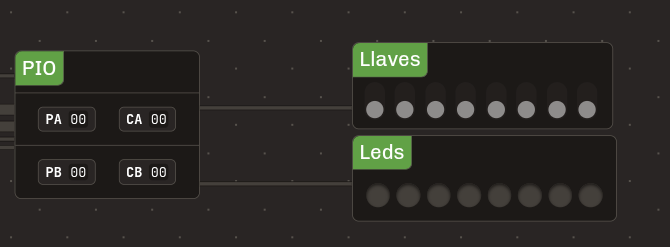
\includegraphics[scale=0.75]{pio0_vonsim.png}
\end{center}
\end{frame}


\subsection{Configuración}
\begin{frame}[fragile]
\frametitle{Configuración del PIO}
\begin{itemize}
  \item Para usar el PIO en esta configuración debemos configurar cada bit del puerto A como entrada y cada bit del puerto B como salida.
\end{itemize}

\begin{block}{Ejemplo}
\begin{verbatim}
MOV AL, 0FFH
OUT 32H, AL
MOV AL, 0
OUT 33H, AL
...
\end{verbatim}

\end{block}

\end{frame}


\section{Impresora}
\subsection{Introducción}
\begin{frame}
\frametitle{Descripción}
\begin{itemize}
  \item La impresora:
  \begin{itemize}
      \item Recibe de un caracter a la vez
      \item Tiene una linea de datos llamada \emph{BUSY} (ocupada) que nos indica si puede recibir un caracter
      \item Tiene una linea de datos llamada \emph{STROBE} que nos permite indicarle a la impresora que queremos enviarle un dato.
      \item La linea de datos \emph{STROBE} debe estar siempre en 0, salvo cuando se envia el pulso, que se envia un 1, y luego vuelve a 0.
      \item Tiene un puerto de 8 bits donde recibe el caracter a imprimir
  \end{itemize}
\end{itemize}
\end{frame}

\begin{frame}
\frametitle{Descripción}
\begin{center}
 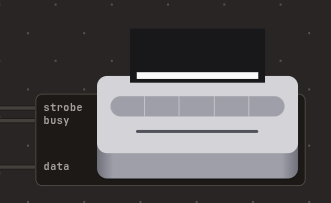
\includegraphics[scale=0.75]{impresora_vonsim.png}
\end{center}
\end{frame}


\begin{frame}
\frametitle{Conexión en el simulador}
  \begin{itemize}
  \item Podemos cambiar la configuración accediendo al menú.
\end{itemize}
\begin{center}
 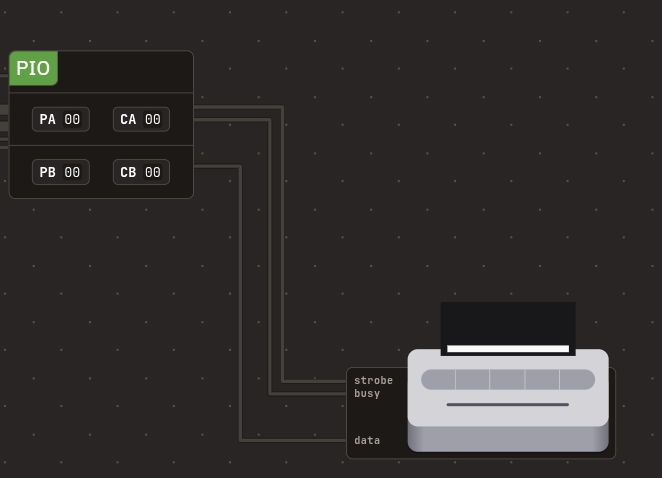
\includegraphics[scale=0.45]{pio1_vonsim.png}
\end{center}
\end{frame}

\subsection{Direccionamiento}
\begin{frame}
\frametitle{Direccionamiento}
La impresora esta conectada de la siguiente manera:
\begin{itemize}
    \item El puerto B del PIO esta conectado al puerto de 8 bits de la impresora, donde recibe el caracter.
    \item El puerto A del PIO esta conectado asi:
\begin{itemize}
    \item Bit 0: BUSY
    \item Bit 1: STROBE
    \item Bit 2..7: Sin conexión
\end{itemize}
\end{itemize}
\end{frame}

\subsection{Uso de la impresora}
\begin{frame}
\frametitle{Uso de la impresora}
Para imprimir debemos:
\begin{itemize}
    \item Inicializar el PIO para conectarse a la impresora
    \item Para cada caracter a imprimir:
\begin{itemize}
    \item Esperar a que la impresora no este ocupada (esperar hasta que BUSY valga 0)
    \item Cargar en el registro de datos el caracter a imprimir
    \item Enviar un pulso strobe (ponemos strobe a 1 y luego a 0)
\end{itemize}
\end{itemize}
\end{frame}

\begin{frame}[fragile]
\frametitle{Inicializar el PIO}
\begin{itemize}
    \item Configurar el puerto A para poder leer \emph{BUSY} y poder escribir \emph{STROBE}
    \item Configurar el puerto B para poder escribir en el puerto de datos de la impresora
    \item Poner a 0 el bit \emph{STROBE} (a continuación)
\end{itemize}
\begin{block}{}
\begin{verbatim}
...
; CA = 1111 1101
MOV AL, 0FDH
OUT CA, AL

; CB = 0000 0000
MOV AL, 0
OUT CB, AL
...
\end{verbatim}
\end{block}
\end{frame}

\begin{frame}[fragile]
\frametitle{Inicializar el PIO (continuación) }
\begin{itemize}
    \item \sout{Configurar el puerto A para poder leer \emph{BUSY} y poder escribir \emph{STROBE}}
    \item \sout{Configurar el puerto B para poder escribir en el puerto de datos de la impresora}
    \item Poner a 0 el bit \emph{STROBE}
\end{itemize}
\begin{block}{}
\begin{verbatim}
...
; Strobe a 0
IN AL, PA 
AND AL, 0FDH
OUT PA, AL
...
\end{verbatim}
\end{block}

\end{frame}


\begin{frame}[fragile]
\frametitle{Esperar a que la impresora no este ocupada}
Leemos la linea BUSY hasta que este en 0
\begin{block}{}
\begin{verbatim}
      ...
POLL: IN AL, PA
      TEST AL, 1
      JNZ POLL
      ...
\end{verbatim}
\end{block}
\end{frame}

\begin{frame}[fragile]
\frametitle{Cargar en el registro de datos el caracter a imprimir}
Cargar el caracter en el puerto B del PIO
\begin{block}{}
\begin{verbatim}
      ...
      MOV AL, PROXIMO_CAR
      OUT PB, AL
      ...
\end{verbatim}
\end{block}
\end{frame}

\begin{frame}[fragile]
\frametitle{Enviar un pulso strobe}
\begin{itemize}
    \item Escribimos un 1 en STROBE
    \item Escribimos un 0 en STROBE
\end{itemize}
\begin{block}{}
\begin{verbatim}
       ...
       ; Strobe a 1
       IN AL, PA
       OR AL, 02H
       OUT PA, AL

       ; Strobe a 0
       IN AL, PA
       AND AL, 0FDH
       OUT PA, AL           
       ...
\end{verbatim}
\end{block}

\end{frame}

\end{document}

